\documentclass[convert={density=900,size=1080x800,outext=.png}]{standalone}
\usepackage{tikz}
\usetikzlibrary{calc, positioning}
\usetikzlibrary{arrows.meta}
\usetikzlibrary{matrix}
\usetikzlibrary{shadows}
\usepgflibrary{shapes.misc}
\usepgflibrary{{shapes.geometric}}
\usetikzlibrary{arrows,positioning,shapes}

\pgfdeclarelayer{shadow} 
\pgfsetlayers{shadow,main}
\def\shadowradius{3pt}


\def\lw{1mm}        % Arrow line width
\def\mw{2cm}        % Minimum width of component
\def\mh{1.75cm}     % Minimum height of component
\def\trianglecoordinate{2mm}    % Starting coordinate clock input triangle of components

\newcommand\drawshadowbis[1]{
    \begin{pgfonlayer}{shadow}
        \fill[inner color=black,outer color=white] ($(#1.south west)$) circle (\shadowradius);
        \fill[inner color=black ,outer color=white] ($(#1.north west)$) circle (\shadowradius);
        \fill[inner color=black ,outer color=white] ($(#1.south east)$) circle (\shadowradius);
        \fill[inner color=black,outer color=white] ($(#1.north east)$) circle (\shadowradius);
        \fill[ top color=black, bottom color=white] ($(#1.south west)+((0,-\shadowradius)$) rectangle ($(#1.south east)$);
        \fill[left color=black,right color=white] ($(#1.south east)$) rectangle ($(#1.north east)+((\shadowradius,0)$);
        \fill[bottom color=black,top color=white] ($(#1.north west)$) rectangle ($(#1.north east)+((0,\shadowradius)$);
        \fill[right color=black,left color=white] ($(#1.south west)$) rectangle ($(#1.north west)+(-\shadowradius,0)$);
    \end{pgfonlayer}
    }

\tikzset{
    border/.style = { 
        draw, rectangle, minimum width=2.5cm, minimum height=2cm, ultra thick
    },
    pics/Component/.style n args={3}{
        code = {
            \node [border, align=center](-edge){#1};
            \draw[thick] ([xshift=\trianglecoordinate] -edge.south) -- ([yshift=\trianglecoordinate] -edge.south);
            \draw[thick] ([xshift=-\trianglecoordinate] -edge.south) -- ([yshift=\trianglecoordinate] -edge.south);
            \draw[thick] (-edge.south) |- ++(-3mm, -4mm) node[xshift=-2mm, yshift=-1mm] {#2}; 
            \draw (-edge.south) node [yshift=-0.75*\mh, align=left, font=\large] {#3};
    }}
    }



\begin{document}
    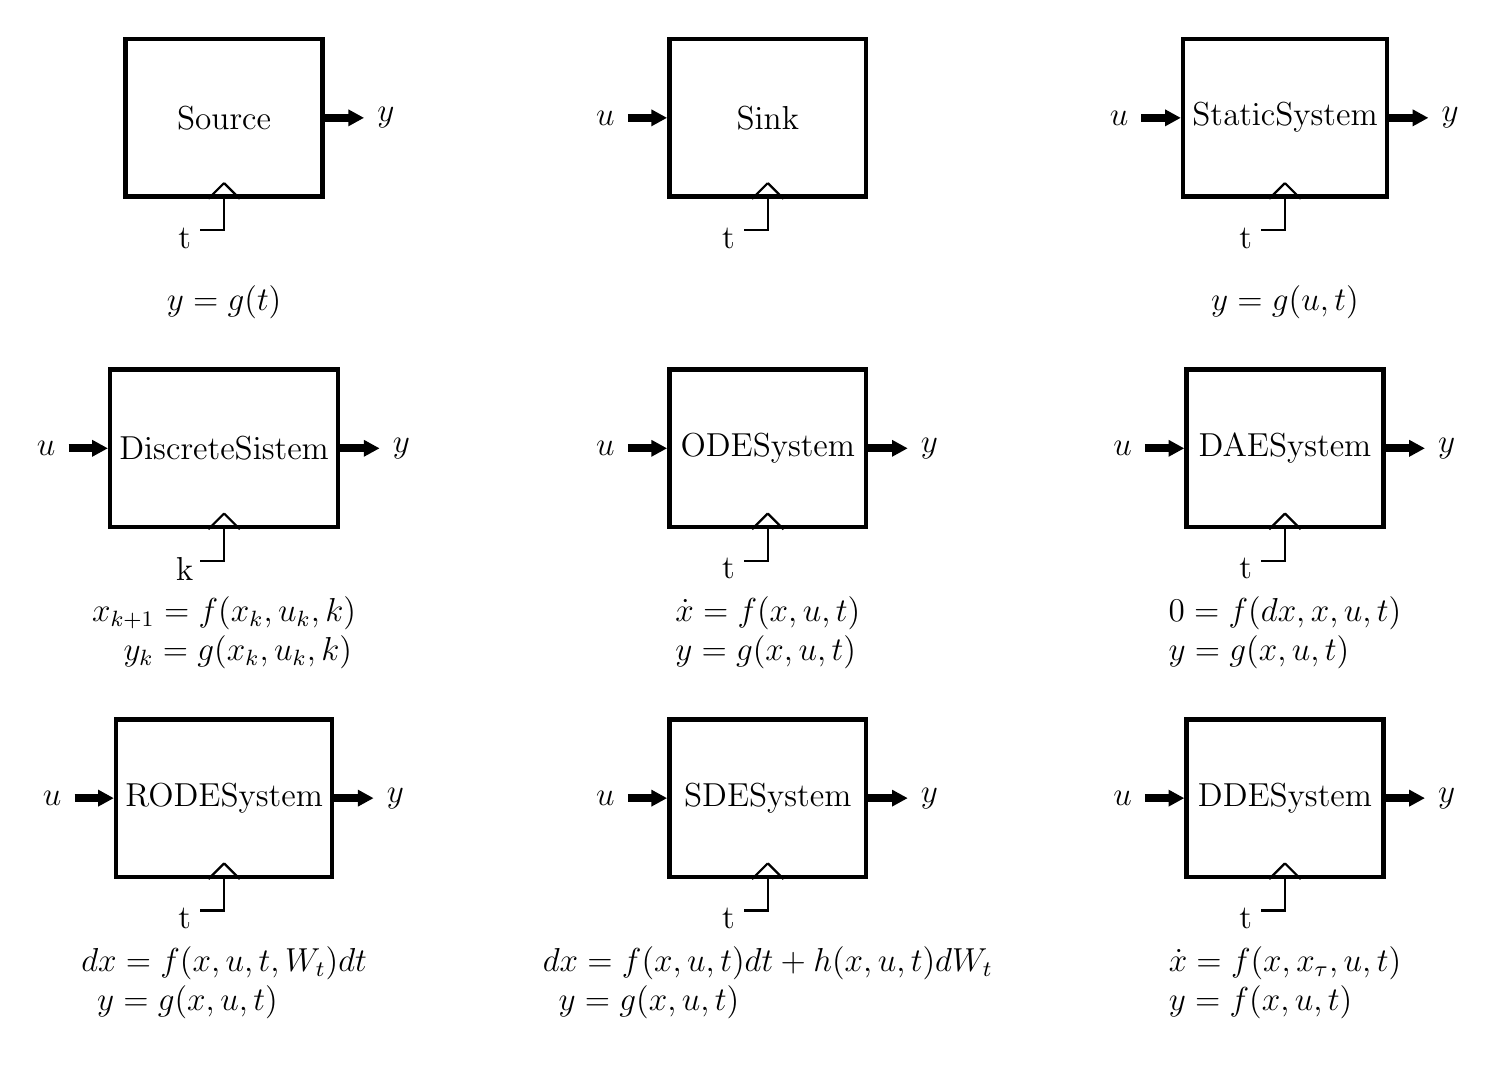
\begin{tikzpicture}[every node/.style={font={\large}}]
        % Place the blocks 
        \matrix (m) [matrix of nodes, ampersand replacement=\&, column sep = 2cm, row sep = 0.5cm, 
            nodes={anchor=center}]{
        \draw pic (b1) {Component={Source}{t}{$y=g(t)$}};    
        \& 
        \draw pic (b3) {Component={Sink}{t}{}};  
        \&
        \draw pic (b5) {Component={StaticSystem}{t}{$y=g(u, t)$}};    
        \\
        \draw pic (b9) {Component={DiscreteSistem}{k}{$x_{k+1}=f(x_k, u_k, k)$\\$\hspace*{0.4cm}y_k=g(x_k, u_k, k)$}};
        \& 
        \draw pic (b7) {Component={ODESystem}{t}{$\dot{x}=f(x,u,t)$\\$y=g(x,u,t)$}};
        \& 
        \draw pic (b2) {Component={DAESystem}{t}{$0=f(dx,x,u,t)$\\$y=g(x,u,t)$}}; 
        \\
        \draw pic (b4) {Component={RODESystem}{t}{$dx=f(x,u,t,W_t)dt$\\$\hspace*{0.2cm}y=g(x,u,t)$}};
        \& 
        \draw pic (b6) {Component={SDESystem}{t}{$dx=f(x,u,t)dt+h(x,u,t)dW_t$\\$\hspace*{0.2cm}y=g(x,u,t)$}};
        \&
        \draw pic (b8) {Component={DDESystem}{t}{$\dot{x}=f(x,x_\tau,u,t)$\\$y=f(x,u,t)$}}; 
        \\
        };
        % % Glow the blocks
        % \foreach \x in {1, 2, ..., 9}{
        %     \drawshadowbis{b\x-edge};
        % }
        \begin{scope}[line width=\lw, >={Triangle[width=2mm,length=2mm]}]
            \foreach \x in {1, 2, 4, 5, 6, 7, 8, 9}{
                \draw[line width = \lw, ->] (b\x-edge.east) -- ++(0.5cm, 0cm) node[anchor=west]{$y$};
            }
            \foreach \x in {2, 3, 4, 5, 6, 7, 8, 9}{
                \draw[line width = \lw, ->] ([xshift=-0.5cm] b\x-edge.west) node[anchor=east]{$u$} -- (b\x-edge.west);
            }
        \end{scope}
    \end{tikzpicture}
\end{document}
